%%Uncomment for lecture version
\documentclass[aspectratio=169]{beamer}
\usepackage{pgfpages}
%\setbeameroption{show notes on second screen=right}
%%Uncomment for handouts
%\documentclass[aspectratio=169, handout]{beamer}
\usepackage{./diegobeamer,mylistings}
\usepackage{datetime2}
\usepackage{tikz}
%\usepackage{marginnote}
% \usepackage{enumitem}
\usetikzlibrary{positioning,decorations.pathreplacing,fit}
%\documentclass[aspectratio=169, notes=only]{beamer}
%\documentclass[notes]{beamer}       % print frame + notes
% Common settings for all lectures in this course
\usepackage{hyperref}
\usepackage{makecell}
\usepackage{array}
\renewcommand\UrlFont{\color{blue}\rmfamily}
\usepackage{amssymb}
\usepackage{amsmath}
\usepackage{numprint}
\usepackage{paralist}
\usepackage{stmaryrd}
\usepackage{listings, xcolor}
\input{solidity_lang}
\DeclareMathOperator{\dsum}{+}
\newcommand{\fromString}[1]{\ensuremath{\left\lceil#1\right\rceil}}
\newcommand{\toString}[1]{\ensuremath{\left\lfloor#1\right\rfloor}}
\newcommand{\update}[3]{
	\ensuremath{#1[#2\mapsto #3]}
}
\newcommand{\option}[1]{
	\ensuremath{#1}_\bot
}
\newcommand{\astack}[1]{\ensuremath{\mathit{sck}(#1)}}
\newcommand{\amemory}[1]{\ensuremath{\mathit{mem}(#1)}}
\newcommand{\astorage}[1]{\ensuremath{\mathit{sto}(#1)}}
\newcommand{\aaccount}[1]{\ensuremath{\mathit{acc}(#1)}}
\newcommand{\ustack}[2]{\ensuremath{\mathit{upSck}(#1,#2)}}
\newcommand{\umemory}[2]{\ensuremath{\mathit{upMem}(#1,#2)}}
\newcommand{\ustorage}[2]{\ensuremath{\mathit{upSto}(#1,#2)}}
\newcommand{\uaccount}[2]{\ensuremath{\mathit{upAcc}(#1,#2)}}
\newcommand{\Mod}[2]{#1~\mathrm{mod}~#2}

\newcommand{\tikzmark}[2][]{%
  \tikz[remember picture,overlay,baseline=-.5ex] \node[#1] (#2) {};%
}
% \drawBrace[xshift]{beginningNode}{endingNode}
% This command draws a brace between two tikzmarks, to their right,
% no matter which one is the rightmost, and includes 
% a node midway the brace, to write the comment.
% This command also creates a new node
% Whose name is the concat of the names of beginning and ending nodes.
\newcommand*{\drawBrace}[4][0pt]{%
    \node[draw=none, fit={(#2) (#3)}, inner sep=0pt] (rectg) {};%
    \draw [decoration={brace,amplitude=0.3em},decorate,very thick,red]%
      ([xshift=#1]rectg.north east) --%
      coordinate[right=.5em, midway] (#2#3)
      ([xshift=#1]rectg.south east);%
    \node[right=.4em of #2#3,align=left] (#2#3-comment) {#4};
    \draw (#2#3-comment.west) edge (#2#3);
}%
\def\lecturename{Computer Languages and Representations}
\def\lecturecode{ECM2418}
\def\coauthor{Achim D. Brucker}

\title{Secure Smart Contracts with Isabelle/Solidity}
%\subtitle{Secure Smart Contracts with Isabelle/Solidity}
\author{Diego Marmsoler, Asad Ahmed, Achim D. Brucker}

\institute
{
  Department of Computer Science\\
  University of Exeter
}

\lecture[1]{Introduction}{introduction}
\date{\DTMdisplaydate{2022}{03}{30}{-1}}
\makeatletter
\def\blfootnote{\gdef\@thefnmark{}\@footnotetext}
\makeatother
\begin{document}
\begin{frame}[plain,noframenumbering]
\maketitle
\bigskip
\bigskip
%\begin{center}
%\includegraphics[width=1.5 in]{logo.PNG}
%\end{center}
\begin{tikzpicture}[remember picture, overlay]
\node[yshift=-3cm] at (current page.center) 
{
    \includegraphics[width=1.5 in]{logo.PNG}
};
\end{tikzpicture}
\end{frame}

\frame{\tableofcontents}

\section{introduction}
\frame{\tableofcontents[currentsection]}

\subsection{Blockchain Technology}

\begin{frame}{Blockchain Technology}
\begin{itemize}
\item A database concept which relies upon decentralization and cryptography to store and retrieve the related database for transparency, immutability and security
\end{itemize}
 \tikz \node at (0, 3) [font=\large,   minimum height=2.5em, minimum width = 3.25cm, inner sep=0pt, fill=blue!30] {Application Layer};
\tikz \node [font=\normalsize, minimum height=2.5em, align = left] {Buisness logic for:\\[0.5pt]  Finance, Medical, Business, Agriculture etc};\\
\tikz \node [font=\large,  minimum height=2.5em, minimum width = 3.25cm, inner sep=0pt, fill=green!30 ] {Contract Layer};
\tikz \node [font=\normalsize, minimum height=2.5em, align = left] {Programs in high-level languages to\\[0.5pt]  implement the buisness logic};\\
\tikz \node [font=\large,  minimum height=2.5em, minimum width = 3.25cm, inner sep=0pt, fill=blue!30] {Consensus layer};
\tikz \node [font=\normalsize, minimum height=2.5em, align = left] {Set of rules agreed upon to add a new block,\\[0.5pt] such as  Proof of Work (PoW)};\\
\tikz \node [font=\large,  minimum height=2.5em, minimum width = 3.25cm, inner sep=0pt, fill=blue!30] {Network Layer};
\tikz \node [font=\normalsize, minimum height=2.5em, align = left] {Handels the communciationa between nodes};\\
\tikz \node [font=\large,  minimum height=2.5em, minimum width = 3.25cm, inner sep=0pt, fill=blue!30] {Data Layer};
\tikz \node [font=\normalsize, minimum height=2.5em, align = left] {Data transections, Blocks, Cryptography};\\
\begin{itemize}
\item High-level programs enlarges the threat surface
\end{itemize}
	%Based on Solidity v0.5.16
	%\bigskip

	%Semantics comes in a \emph{denotational style}
	%\begin{equation*}
	%	\mathcal{S}\colon~\mathbf{S}\to\mathbf{Env}_\mathbf{p}\to\mathbf{Env}_\mathbf{v}\to\mathbf{Calldata}\to\mathbf{StateMonad}
	%\end{equation*}\vspace{-.5cm}

	%\begin{columns}[T]
	%	\column{.43\textwidth}
	%	Formalized in Isabelle/HOL
	%	\begin{itemize}
	%		\item Deep embedding
	%		\item Executable
	%	\end{itemize}
		
	%	\column{.53\textwidth}
	%	\includegraphics[width=\columnwidth]{./img/value.PNG}
	%\end{columns}
\end{frame}
\subsection{Contract Layer}
\begin{frame}{Smart Contracts}

 \begin{itemize}
\item Programs wirtten in high-level languages, such as Solidity, C etc
\item Allows to automate the transections in a Blockchain
\item Key feature is: once deployed cannot be modified
\item Errors and bugs in the smart contract programs lead to unbearable finanical losses
\end{itemize}
	%Based on Solidity v0.5.16
	%\bigskip

	%Semantics comes in a \emph{denotational style}
	%\begin{equation*}
	%	\mathcal{S}\colon~\mathbf{S}\to\mathbf{Env}_\mathbf{p}\to\mathbf{Env}_\mathbf{v}\to\mathbf{Calldata}\to\mathbf{StateMonad}
	%\end{equation*}\vspace{-.5cm}

	%\begin{columns}[T]
	%	\column{.43\textwidth}
	%	Formalized in Isabelle/HOL
	%	\begin{itemize}
	%		\item Deep embedding
	%		\item Executable
	%	\end{itemize}
		
	%	\column{.53\textwidth}
	%	\includegraphics[width=\columnwidth]{./img/value.PNG}
	%\end{columns}
\end{frame}


\begin{frame}{Decentralized Autonomous Organization (DAO) smart contract}

 \begin{itemize}
\item Infamous malicious attack took place in 2016 
\item (DAO) smart contract was manipulated to steal around 2 Million Ether
\item Re-entrancy vulnerability
\end{itemize}
\end{frame}

\begin{frame}{Related Work}
\begin{tabular}{ccccc}
					 & \textbf{\small Tool} 		& \textbf{\small Approach}	 			& \textbf{\small Formal Methods}	 					& \textbf{\small Language}  \\
\hline
\makecell{\small {Bhargavan et al.} \\ \small{2016}} 		& \makecell{\small{Solidity$^{*}$} \\ \small{\& EVM$^{*}$}}		& \small{Axiometic}	 	& \small{SMT}				& \small{F$^{*}$}\\
\hline
\makecell{ \small{Ahrendt et al.}\\ \small{2016}} 					& \small{SoliditiKeY}						& \small{Axiometic}	 	& \small{KeY}				& \small{DL}\\
\hline
\makecell{\small{Hajdu et al.}\\ \small{2019,20}}						&\small{SOLC-VERIFY}					&\small{Axiometic}		&\small{SMT}				&\small{Boogie}\\
\hline
\makecell{\small{Tai et al.}\\ \small{2023}}						&\small{iCONTRACT}						&\small{Axiometic}		&\small{SMT}				&\small{Python}\\
\hline
\makecell{\small{Jiao et al.}\\ \small{2020}} 						&\textemdash\							& \small{Axiomatic}		& \small{Model Checking}	& \small{K}\\
\hline
\makecell{\small{Diego et al.}\\ \small{2021}}				& \textemdash\ 							&\small{by-construciton}	&\small{Theorem Proving}	&\small{HOL}\\
\hline
\makecell{\small{Ribeiro et al.} \\ \small{2020}}	& \small{SOLI}							&\small{by-construction}	&\small{Theorem Proving}	&\small{HOL}\\
\hline
\end{tabular}
%\begin{tabular}{ccccc}
%					 & \textbf{\small Tool} 		& \textbf{\small Approach}	 			& \textbf{\small Formal Methods}	 					& \textbf{\small Language}  \\
%\hline
%\makecell{\small {Bhargavan et al.\\(2016)}} 		& \small{Solidity$^{*}$ \& EVM$^{*}$}		& \small{Axiometic}	 	& \small{SMT}				& \small{F$^{*}$}\\
%\hline
%\makecell{ \small{Ahrendt et al.\\(2016)}} 					& \small{SoliditiKeY}						& \small{Axiometic}	 	& \small{KeY}				& \small{DL}\\
%\hline
%\makecell{\small{Hajdu et al.\\(2019,20)}}						&\small{SOLC-VERIFY}					&\small{Axiometic}		&\small{SMT}				&\small{Boogie}\\
%\hline
%\makecell{\small{Tai et al.}}						&\small{iCONTRACT}						&\small{Axiometic}		&\small{SMT}				&\small{Python}\\
%\hline
%\makecell{\small{Jiao et al.}} 						&\textemdash\							& \small{Axiomatic}		& \small{Model Checking}	& \small{K}\\
%\hline
%\makecell{\small{Diego et al.\small}}				& \textemdash\ 							&\small{by-construciton}	&\small{Theorem Proving}	&\small{HOL}\\
%\hline
%\makecell{\small{Ribeiro et al.} \\ \small{(2020)}}	& \small{SOLI}							&\small{by-construction}	&\small{Theorem Proving}	&\small{HOL}\\
%\hline
%\end{tabular}
%\begin{figure}
%\centering
%\begin{tabular}{cl}
%%
%    \includegraphics[width=2cm]{pimage.png} & \begin{minipage}[t]{0.75\textwidth} 
%Bhargavan, K., et.al.: Formal verification of smart contracts: Short paper. In: Programming
%Languages and Analysis for Security. pp. 91–96. PLAS, ACM (2016)
%\end{minipage}
% \\ 
%%
%    \includegraphics[width=2cm]{pimage.png} & C\begin{minipage}[t]{0.75\textwidth} 
%Bhargavan, K., et.al.: Formal verification of smart contracts: Short paper. In: Programming
%Languages and Analysis for Security. pp. 91–96. PLAS, ACM (2016)
%\end{minipage}\\ 
%%
%    B & D \\ 
%%
%\end{tabular}
%\end{figure}
 %\begin{itemize}
%\item 
%\end{itemize}
\end{frame}
%
%\subsection{Proposed Methodology}
%\begin{frame}{Proposed Methodology}
%\begin{figure}[!h]
%\centering
%\begin{tikzpicture}
%%PICTURE SCOPE or REFERENCEs
%\node at (0, 0) (topleft) [circle] {};
%%\node at (11.75, 0) (topright) [circle, draw=red, fill=red] {};
%\node (topright) [circle, xshift = 10.5cm, right of = topleft] {};
%\node (bottomleft) [circle, yshift = -7.25cm, below of = topleft] {};
%\node (bottomright) [circle, xshift = 11.5cm, yshift = -7.25cm, below of = topleft] {};
%%\draw (0,-3) [draw=red, fill=red]  -- (5, -4); % CHECK once of the grid is affecting the placement of the objects
%%GRID
%
%\draw (2, -0.45 ) [rounded corners = 4pt, draw=black, fill=blue!4]  -- ++(6.5cm, 0) --++(0, -7.35cm)--++(-6.5, 0)--cycle;
%\draw (2.5, -0.65) [rounded corners = 4pt, draw=black, fill=blue!4]  -- ++(5cm, 0) --++(0, -2.65cm)--++(-5, 0)--cycle;
%\draw (2.65, -0.85) [rounded corners = 4pt, draw=black, fill=blue!4]  -- ++(3.1cm, 0) --++(0, -2.3cm)--++(-3.1, 0)--cycle;
%%INPUTS
%\node (solidity) [thin, draw=black, fill=red!4,  rectangle, rounded corners= 2pt, xshift = 3.5cm, right of = topleft, inner sep = 4pt] {\scriptsize Solidity (v 0.8.25)};
%\node (sc) [thin, draw=black, fill=red!4,  rectangle, rounded corners= 2pt, yshift = -4.75cm, right of = topleft, inner sep = 4pt, align = center] {\scriptsize Smart \\[0.15pt] \scriptsize Contract};
%\node (scp) [thin, draw=black, fill=red!4,  rectangle, rounded corners= 2pt, xshift = -0.35cm, yshift = -7.10cm, right of = topleft, inner sep = 4pt, align = center] {\scriptsize Property  \\[0.15pt] \scriptsize  Specification \scriptsize \& \\[0.15pt]  \scriptsize  Verification};
%%THEORIES
%\node (thy1) [thin, draw=black, fill=blue!4,  rectangle, rounded corners= 2pt, xshift = -1.3cm, yshift= -1.25cm, right of = solidity, inner sep = 4pt] {\scriptsize State.thy};
%\node (thy2) [thin, draw=black, fill=blue!4,  rectangle, rounded corners= 2pt, xshift = -1.3cm, yshift= -2cm, right of = solidity, inner sep = 4pt] {\scriptsize State\_monad.thy};
%\node (thy3) [thin, draw=black, fill=blue!4,  rectangle, rounded corners= 2pt, xshift = -1.3cm, yshift= -2.75cm, right of = solidity, inner sep = 4pt] {\scriptsize Solidity.thy};
%\node (thy4) [thin, draw=black, fill=blue!4,  rectangle, rounded corners= 2pt, xshift = 1.15cm, yshift= -2.75cm, right of = solidity, inner sep = 4pt] {\scriptsize WP.thy};
%%ISASOLISITY
%\node (isasolidity) [thin, draw=black, fill=blue!4,  rectangle, rounded corners= 2pt, xshift = -1.75cm, yshift= -4.75cm, right of = solidity, inner sep = 4pt, align = center] {\scriptsize Isabelle/Solidity  \\[0.15pt] \scriptsize Specification};
%\node (isaver) [thin, draw=black, fill=blue!4,  rectangle, rounded corners= 2pt, xshift = -1.35cm, yshift= -6.1cm, right of = solidity, inner sep = 4pt, align = center] { \scriptsize  Verification Keywords};
%\node (vcg) [thin, draw=black, fill=blue!4,  rectangle, rounded corners= 2pt, xshift = -1cm, yshift= -7.20cm, right of = solidity, inner sep = 4pt, align = center] {\scriptsize  Verification Code Generator};
%%ISAHOL
%\node (dtl) [thin, draw=black, fill=blue!4,  rectangle, rounded corners= 2pt, xshift = 2.25cm,  yshift= -5.65cm, right of = solidity, inner sep = 4pt,   align = center, rotate=90] { {\scriptsize Isabelle/HOL}\\[0.15] {\scriptsize  Definitions/Thoerems/Lemmas}};
%\node (isac) [thin, draw=black, fill=blue!4,  rectangle, rounded corners= 2pt, minimum width= 6cm, xshift = 4cm,  yshift= -4cm, right of = solidity, inner sep = 4pt,   align = center, rotate=90] { {\scriptsize Isabelle/HOL Core}};
%\node (vsc) [thin, draw=black, fill=green!10,  rectangle, rounded corners= 2pt, minimum width= 6cm, xshift = 5.5cm,  yshift= -4cm, right of = solidity, inner sep = 4pt,   align = center, rotate=90] { {\scriptsize Verified Smart Contract}};
%%CONNECTING ARROWS
%%%INPUT ARROWS HORIZENTAL
%%\draw  [draw=black, line width = 1.5pt, ->] (sc.east) to [ out=360, in=180] ++(0.65cm,0);;
%%
%\draw  [draw=black, line width = 1.5pt, ->] (sc.east) to [ out=360, in=180] (isasolidity.west);;
%%
%\draw  [draw=black, line width = 1.5pt, <-] (vcg.west) to [ out=-180, in=0] ++(-0.88cm, 0);;
%%\draw  [draw=black, line width = 1.5pt, ->] (scp.north) to [ out=90, in=180] ++(0, 0.15cm) |- (isaver.west);;
%\draw  [draw=black, line width = 1.5pt, ->] (scp.north) to [ out=90, in=270] ++(0, 0.25cm) |- (isaver.west);;
%%%SC AND VERI VERTICAL CONNNECTORS
%\draw  [draw=black, line width = 1.5pt, <-] (isasolidity.north) -- ++(0, 1.08cm);;
%%
%\draw  [draw=black, line width = 1.5pt, <-] (isaver.north east) -- ++(0, 2.68cm);;
%%
%\draw  [draw=black, line width = 1.5pt, <-] (vcg.north east) -- ++(0, 3.95cm);;
%%
%\draw  [draw=black, line width = 1.5pt, <->] (isasolidity.south) -- ++(0, -0.55cm);;
%%
%\draw  [draw=black, line width = 1.5pt, <->] (vcg.north) -- ++(0, 0.58cm);;
%%
%\draw  [draw=black, line width = 1.5pt, ->] (isasolidity.east) -- ++(2.35cm, 0);;
%%
%\draw  [draw=black, line width = 1.5pt, ->] (isaver.east) -- ++(1.6cm, 0);;
%%
%\draw  [draw=black, line width = 1.5pt, ->] (vcg.east) -- ++(0.85cm, 0);;
%%\draw [thick, <->, >=open triangle 45]  (dummyhv.south) -- ++(0, -0.85cm) |- node [near end] {} (HOLLIGHT);
%%\draw  [draw=black, line width = 1.5pt, ->] (dtl.north) -- ++(-1.15cm, 0) |- --++(0, -0.5cm);
%%\draw  [draw=black, line width = 1.5pt, ->] (dtl.north) to [ out=90, in=-270] -- ++(0, 0.5cm) ;;
%%\draw  [draw=black, line width = 1.5pt, <->] (7.20, -5.5) -- ++(-0.5cm, 0)  |- node [near end] {} (6.70, -3.30);;
%\draw  [draw=black, line width = 1.5pt, <-] (6.70, -3.30) -- ++(0, -2cm) ;;
%\draw  [draw=black, line width = 1.5pt, ->] (6.70, -5.27) -- ++(0.52cm, 0) ;;
%%DTL to CORE
%\draw  [draw=black, line width = 1.5pt, <->] (8.27, -5.30) -- ++(0.95cm, 0) ;;
%%Theories to core
%\draw  [draw=black, line width = 1.5pt, <->] (7.5, -2.30) -- ++(1.7cm, 0) ;;
%%CORE TO VERIFICATION
%\draw  [draw=black, line width = 1.5pt, ->] (isac.south) --(vsc.north) ;;
%%SOLIDITY TO THY
%\draw  [draw=black, line width = 1.5pt, ->] (solidity.south) --  ++(0, -0.35cm) ;;
%
%
%\end{tikzpicture}
%\end{figure}
%\end{frame}
\begin{frame}{Problem Statement}
\end{frame}
\subsection{Proposed Methodology}
\begin{frame}{Proposed Methodology}
\begin{figure}[!h]
\centering
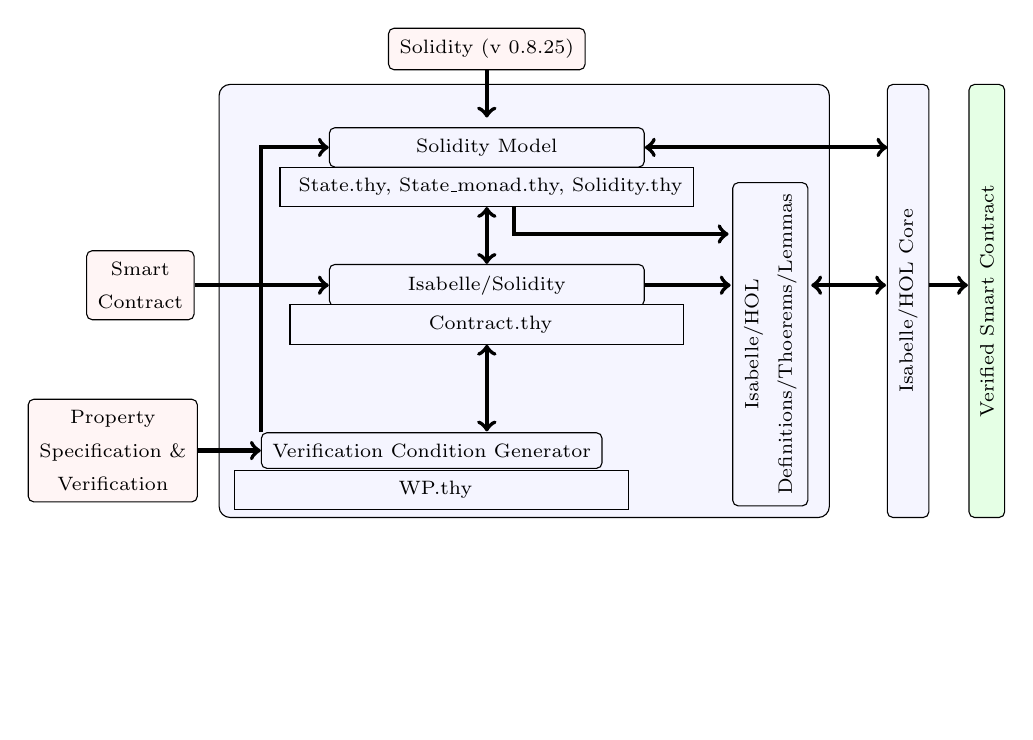
\begin{tikzpicture}
%PICTURE SCOPE or REFERENCEs
\node at (0, 0) (topleft) [circle] {};
%\node at (11.75, 0) (topright) [circle, draw=red, fill=red] {};
\node (topright) [circle, xshift = 10.5cm, right of = topleft] {};
\node (bottomleft) [circle, yshift = -7.25cm, below of = topleft] {};
\node (bottomright) [circle, xshift = 11.5cm, yshift = -7.25cm, below of = topleft] {};
%\draw (0,-3) [draw=red, fill=red]  -- (5, -4); % CHECK once of the grid is affecting the placement of the objects
%GRID

\draw (2, -0.45 ) [rounded corners = 4pt, draw=black, fill=blue!4]  -- ++(7.75cm, 0) --++(0, -5.5cm)--++(-7.75, 0)--cycle;
%\draw (2.5, -0.65) [rounded corners = 4pt, draw=black, fill=blue!4]  -- ++(5cm, 0) --++(0, -2.65cm)--++(-5, 0)--cycle;
%\draw (2.65, -0.85) [rounded corners = 4pt, draw=black, fill=blue!4]  -- ++(3.1cm, 0) --++(0, -2.3cm)--++(-3.1, 0)--cycle;
%INPUTS
\node (solidity) [thin, draw=black, fill=red!4,  rectangle, rounded corners= 2pt, xshift = 4.40cm, right of = topleft, inner sep = 4pt] {\scriptsize Solidity (v 0.8.25)};
\node (sc) [thin, draw=black, fill=red!4,  rectangle, rounded corners= 2pt, yshift = -3cm, right of = topleft, inner sep = 4pt, align = center] {\scriptsize Smart \\[0.15pt] \scriptsize Contract};
\node (scp) [thin, draw=black, fill=red!4,  rectangle, rounded corners= 2pt, xshift = -0.35cm, yshift = -5.10cm, right of = topleft, inner sep = 4pt, align = center] {\scriptsize Property  \\[0.15pt] \scriptsize  Specification \scriptsize \& \\[0.15pt]  \scriptsize  Verification};
%%THEORIES
\node (sm) [thin, draw=black, fill=blue!4,  rectangle, minimum width=4cm, rounded corners= 2pt, xshift = 4.40cm, yshift = -1.25cm, right of = topleft, inner sep = 4pt, align = center] {\scriptsize Solidity Model};
\node (sm1) [thin, draw=black, fill=blue!4,  rectangle, minimum width=4cm,  xshift = 4.40cm, yshift = -1.75cm, right of = topleft, inner sep = 4pt, align = center] {\scriptsize{ State.thy, State\_monad.thy, Solidity.thy}};
%
\node (isasol) [thin, draw=black, fill=blue!4,  rectangle, minimum width=4cm, rounded corners= 2pt, xshift = 4.40cm, yshift = -3cm, right of = topleft, inner sep = 4pt, align = center] {\scriptsize Isabelle/Solidity};
\node (isasol1) [thin, draw=black, fill=blue!4,  rectangle, minimum width=5cm,  xshift = 4.40cm, yshift = -3.50cm, right of = topleft, inner sep = 4pt, align = center] {\scriptsize{ Contract.thy}};
%
\node (vcg) [thin, draw=black, fill=blue!4,  rectangle, minimum width=4cm, rounded corners= 2pt, xshift = 3.70cm, yshift = -5.10cm, right of = topleft, inner sep = 4pt, align = center] {\scriptsize Verification Condition Generator};
\node (vcg1) [thin, draw=black, fill=blue!4,  rectangle, minimum width=5cm, xshift = 3.70cm, yshift = -5.60cm, right of = topleft, inner sep = 4pt, align = center] {\scriptsize{ WP.thy}};
%
\node (dtl) [thin, draw=black, fill=blue!4,  rectangle, minimum width=4cm, rounded corners= 2pt, xshift = 8cm, yshift = -3.75cm, right of = topleft, inner sep = 4pt, align = center, rotate=90] { {\scriptsize Isabelle/HOL}\\[0.15] {\scriptsize  Definitions/Thoerems/Lemmas}};
\node (isac) [thin, draw=black, fill=blue!4,  rectangle, rounded corners= 2pt, minimum width= 5.5cm, xshift = 9.75cm,  yshift= -3.2cm, right of = topleft,  inner sep = 4pt,   align = center, rotate=90] { {\scriptsize Isabelle/HOL Core}};
\node (vsc) [thin, draw=black, fill=green!10,  rectangle, rounded corners= 2pt, minimum width= 5.5cm, xshift = 10.75cm,  yshift= -3.2cm, right of = topleft,  inner sep = 4pt,   align = center, rotate=90] { {\scriptsize Verified Smart Contract}};
%%CONNECTIONS
\draw  [draw=black, line width = 1.5pt, ->] (sc.east) to [ out=360, in=180] (isasol.west);;
\draw  [draw=black, line width = 1.5pt, ->] (scp.east) to [ out=360, in=180] (vcg.west);;
%%INTERCONECTIONS
\draw  [draw=black, line width = 1.5pt, ->] (solidity.south) --  ++(0, -0.60cm) ;;
\draw  [draw=black, line width = 1.5pt, <->] (sm1.south)  to [out=270, in=90] (isasol.north);; ;;
\draw  [draw=black, line width = 1.5pt, <->] (isasol1.south)  to [out=270, in=90] ++(0, -1.10);; ;;
%%SM1 TO DTL
\draw  [draw=black, line width = 1.5pt, ->] (5.75, -2.35) -- ++(2.72cm, 0) ;;
\draw  [draw=black, line width = 1.5pt, -] (5.75, -2) -- ++(0, -0.38cm) ;;
\draw  [draw=black, line width = 1.5pt, ->] (isasol.east) -- ++(1.09cm, 0);;
%%SM TO HOL CORE
\draw  [draw=black, line width = 1.5pt, <->] (sm.east)  -- ++(3.08cm, 0);;;; ;;
%DTL TO CORE
\draw  [draw=black, line width = 1.5pt, <->] (9.52, -3) -- ++(0.95cm, 0) ;;
%%
\draw  [draw=black, line width = 1.5pt, ->] (11.01, -3) -- ++(0.5cm, 0) ;;
%%
\draw  [draw=black, line width = 1.5pt, ->] (vcg.north west) to [out=90, in=-90]   ++(0, 0.38cm)|- (sm.west) ;;

%\draw  [draw=black, line width = 1.5pt, ->] (vcg.north west) to [out=90, in=-90] |- ++(0, 0.38cm) ;;
%\node (thy1) [thin, draw=black, fill=blue!4,  rectangle, rounded corners= 2pt, xshift = -1.3cm, yshift= -1.25cm, right of = solidity, inner sep = 4pt] {\scriptsize State.thy};
%\node (thy2) [thin, draw=black, fill=blue!4,  rectangle, rounded corners= 2pt, xshift = -1.3cm, yshift= -2cm, right of = solidity, inner sep = 4pt] {\scriptsize State\_monad.thy};
%\node (thy3) [thin, draw=black, fill=blue!4,  rectangle, rounded corners= 2pt, xshift = -1.3cm, yshift= -2.75cm, right of = solidity, inner sep = 4pt] {\scriptsize Solidity.thy};
%\node (thy4) [thin, draw=black, fill=blue!4,  rectangle, rounded corners= 2pt, xshift = 1.15cm, yshift= -2.75cm, right of = solidity, inner sep = 4pt] {\scriptsize WP.thy};
%%ISASOLISITY
%\node (isasolidity) [thin, draw=black, fill=blue!4,  rectangle, rounded corners= 2pt, xshift = -1.75cm, yshift= -4.75cm, right of = solidity, inner sep = 4pt, align = center] {\scriptsize Isabelle/Solidity  \\[0.15pt] \scriptsize Specification};
%\node (isaver) [thin, draw=black, fill=blue!4,  rectangle, rounded corners= 2pt, xshift = -1.35cm, yshift= -6.1cm, right of = solidity, inner sep = 4pt, align = center] { \scriptsize  Verification Keywords};
%\node (vcg) [thin, draw=black, fill=blue!4,  rectangle, rounded corners= 2pt, xshift = -1cm, yshift= -7.20cm, right of = solidity, inner sep = 4pt, align = center] {\scriptsize  Verification Code Generator};
%%ISAHOL
%\node (dtl) [thin, draw=black, fill=blue!4,  rectangle, rounded corners= 2pt, xshift = 2.25cm,  yshift= -5.65cm, right of = solidity, inner sep = 4pt,   align = center, rotate=90] { {\scriptsize Isabelle/HOL}\\[0.15] {\scriptsize  Definitions/Thoerems/Lemmas}};
%\node (isac) [thin, draw=black, fill=blue!4,  rectangle, rounded corners= 2pt, minimum width= 6cm, xshift = 4cm,  yshift= -4cm, right of = solidity, inner sep = 4pt,   align = center, rotate=90] { {\scriptsize Isabelle/HOL Core}};
%\node (vsc) [thin, draw=black, fill=green!10,  rectangle, rounded corners= 2pt, minimum width= 6cm, xshift = 5.5cm,  yshift= -4cm, right of = solidity, inner sep = 4pt,   align = center, rotate=90] { {\scriptsize Verified Smart Contract}};
%%CONNECTING ARROWS
%%%INPUT ARROWS HORIZENTAL
%%\draw  [draw=black, line width = 1.5pt, ->] (sc.east) to [ out=360, in=180] ++(0.65cm,0);;
%%
%\draw  [draw=black, line width = 1.5pt, ->] (sc.east) to [ out=360, in=180] (isasolidity.west);;
%%
%\draw  [draw=black, line width = 1.5pt, <-] (vcg.west) to [ out=-180, in=0] ++(-0.88cm, 0);;
%%\draw  [draw=black, line width = 1.5pt, ->] (scp.north) to [ out=90, in=180] ++(0, 0.15cm) |- (isaver.west);;
%\draw  [draw=black, line width = 1.5pt, ->] (scp.north) to [ out=90, in=270] ++(0, 0.25cm) |- (isaver.west);;
%%%SC AND VERI VERTICAL CONNNECTORS
%\draw  [draw=black, line width = 1.5pt, <-] (isasolidity.north) -- ++(0, 1.08cm);;
%%
%\draw  [draw=black, line width = 1.5pt, <-] (isaver.north east) -- ++(0, 2.68cm);;
%%
%\draw  [draw=black, line width = 1.5pt, <-] (vcg.north east) -- ++(0, 3.95cm);;
%%
%\draw  [draw=black, line width = 1.5pt, <->] (isasolidity.south) -- ++(0, -0.55cm);;
%%
%\draw  [draw=black, line width = 1.5pt, <->] (vcg.north) -- ++(0, 0.58cm);;
%%
%\draw  [draw=black, line width = 1.5pt, ->] (isasolidity.east) -- ++(2.35cm, 0);;
%%
%\draw  [draw=black, line width = 1.5pt, ->] (isaver.east) -- ++(1.6cm, 0);;
%%
%\draw  [draw=black, line width = 1.5pt, ->] (vcg.east) -- ++(0.85cm, 0);;
%%\draw [thick, <->, >=open triangle 45]  (dummyhv.south) -- ++(0, -0.85cm) |- node [near end] {} (HOLLIGHT);
%%\draw  [draw=black, line width = 1.5pt, ->] (dtl.north) -- ++(-1.15cm, 0) |- --++(0, -0.5cm);
%%\draw  [draw=black, line width = 1.5pt, ->] (dtl.north) to [ out=90, in=-270] -- ++(0, 0.5cm) ;;
%%\draw  [draw=black, line width = 1.5pt, <->] (7.20, -5.5) -- ++(-0.5cm, 0)  |- node [near end] {} (6.70, -3.30);;
%\draw  [draw=black, line width = 1.5pt, <-] (6.70, -3.30) -- ++(0, -2cm) ;;
%\draw  [draw=black, line width = 1.5pt, ->] (6.70, -5.27) -- ++(0.52cm, 0) ;;
%%DTL to CORE
%\draw  [draw=black, line width = 1.5pt, <->] (8.27, -5.30) -- ++(0.95cm, 0) ;;
%%Theories to core
%\draw  [draw=black, line width = 1.5pt, <->] (7.5, -2.30) -- ++(1.7cm, 0) ;;
%%CORE TO VERIFICATION
%\draw  [draw=black, line width = 1.5pt, ->] (isac.south) --(vsc.north) ;;
%%SOLIDITY TO THY
%\draw  [draw=black, line width = 1.5pt, ->] (solidity.south) --  ++(0, -0.35cm) ;;


\end{tikzpicture}
\end{figure}
\end{frame}


\section{Solidity}
\frame{\tableofcontents[currentsection]}

%\begin{frame}{Bank}
%\begin{itemize}
%\item Keeps an internal record of funds transferred by its customers.
%\item This record is increased whenever a customer transfers additional funds 
%\item When customer withdraws all its recorded
%funds are returned and its internal record reset to 0.
%\end{itemize}
\subsection{Solidity Smart Contract}

\begin{frame}{Solidity Smart Contract}

\begin{soliditybox}
pragma solidity >=0.5.1 <0.5.2;

contract Bank {
    mapping(address => uint256) balances;

    function deposit() public payable {
        balances[msg.sender] = balances[msg.sender] + msg.value;
    }

    function withdraw() public {
        uint256 bal = balances[msg.sender];
        balance[msg.sender] = 0;
        msg.sender.transfer(bal);
    }
}
\end{soliditybox}

	%\begin{center}
	%\includegraphics[width=10cm]{testing}
	%\end{center}
	%\blfootnote{DM and A.D.~Brucker.\\ Conformance Testing of Formal Semantics using Grammar-based Fuzzing. Sub. to TAP 2022.}
\end{frame}

\subsection{Semantic}

\begin{frame}[fragile]{Example}
	\begin{lstlisting}[style=solidity_style, escapechar=!, basicstyle=\tiny, mathescape]
contract TestContract0 {
    uint8 v_u8_s8;!\tikzmark{bgnSVar}!
    mapping(uint16 => uint8) v_m_u16_u8_9;
    bool[1][2] a_b_12_s5;
    ...!\tikzmark{trmSVar}!
    function test() public {
        uint104 v_u104_m2;!\tikzmark{bgnMVar}!
        uint104[1][1] memory a_u104_11_m2;
        ...!\tikzmark{trmMVar}!
        v_u104_m2=14622709355569675963178665339646;!\tikzmark{bgnState}!
        v_m_u16_u8_9[59381]=79;
        ...!\tikzmark{trmState}!
        int8 counter1=int8(0);!\tikzmark{bgnCode}!
        while((v_m_u224_s240_1[uint224(444)]==(v_u216_s1-v_u104_m2)) && counter1<int8(10)){
            0xf7218C33533a3F22e3296F8b1DC0074B399355Eb.transfer(v_m_u16_u8_9[uint16(0)]);
            counter1=counter1+int8(1);
        }
        ...!\tikzmark{trmCode}!
        Assert.equal(v_m_u16_u8_9[59381]==79, true);!\tikzmark{bgnAss}!
        Assert.equal(a_u104_11_m2[0][0]==8130097819054169632795960896007, true);
        Assert.equal(0xf7218C33533a3F22e3296F8b1DC0074B399355Eb
            .balance==100000000000000000000, true);
        ...!\tikzmark{trmAss}!
    }
}!\mbox{%
\begin{tikzpicture}[overlay, remember picture]
    \drawBrace[3cm]{bgnSVar}{trmSVar}{Extracted\\ storage variables};
    \drawBrace[3cm]{bgnMVar}{trmMVar}{Extracted\\ memory/stack variables};
    \drawBrace[1cm]{bgnState}{trmState}{Generated\\ input state};
    \drawBrace[7cm]{bgnCode}{trmCode}{Generated\\ program};
    \drawBrace[4cm]{bgnAss}{trmAss}{Computed \\ result state};
  \end{tikzpicture}}!
\end{lstlisting}
  

\end{frame}

\section{Example Applications}
\frame{\tableofcontents[currentsection]}

\subsection{Verified Constant Solving}
\begin{frame}{Verified Constant Solving}
\begin{columns}
\column{.48\textwidth}
\begin{soliditybox}
int16 x;

// costs 20 Gas
x = int16(250) + uint8(500);

// costs 8 Gas
x = int16(494);
\end{soliditybox}

\bigskip\pause

\begin{center}
We implemented a constant solver for Solidity in Isabelle/HOL and verified that it preserves the semantic of a program.
\end{center}

\column{.48\textwidth}
\includegraphics[width=\columnwidth]{isacs}
\end{columns}
\end{frame}

\subsection{Verification of Simple Token}
\begin{frame}{Functional Verification of (very) Simple Token}
\begin{soliditybox}
pragma solidity >=0.5.1 <0.5.2;

contract Bank {
    mapping(address => uint256) balances;

    function deposit() public payable {
        balances[msg.sender] = balances[msg.sender] + msg.value;
    }

    function withdraw() public {
        uint256 bal = balances[msg.sender];
        balance[msg.sender] = 0;
        msg.sender.transfer(bal);
    }
}
\end{soliditybox}
\end{frame}

\begin{frame}{Functional Verification of (very) Simple Token}
	For both methods we verified the following pre- / postconditions:
	\begin{align*}
		\mathit{pre(\alert{b})}\colon&\mathit{\color{blue}balance}-\sum_{\{(a,x)|\texttt{balances}(a)=x\}} x \geq \mathit{\alert{b}}\\
		\mathit{post(\alert{b})}\colon&\mathit{\color{blue}balance}-\sum_{\{(a,x)|\texttt{balances}(a)=x\}} x \geq \mathit{\alert{b}}
	\end{align*}
\pause

	Note that withdraw triggers the execution of fallback methods which is code we do \emph{not} know yet
	\begin{itemize}
		\item In particular we verified that the above holds \emph{for every possible implementation} of fallback methods
		\item This is possible with Isabelle using structural induction over the implementation of the fallback method
	\end{itemize}
\end{frame}

\section{Conclusion}
\frame{\tableofcontents[currentsection]}

\begin{frame}{Conclusion}
Summary
\begin{itemize}
	\item Deep embedding of subset of Solidity in Isabelle/HOL
	\item Executable semantics with automatic conformance testing
	\item Used to create verified tools for Solidity
	\item Used to verify concrete Solidity contracts
\end{itemize}
\bigskip\pause

Limitations: Semantics
\begin{itemize}
	\item Some advanced features are still missing: inheritance
	\item Based on v0.5.16
\end{itemize}
\bigskip\pause

Limitations: Verification
\begin{itemize}
	\item Reasoning from semantic definitions is tedious
	\item Low degree of automation
	\item Example: Simple token required more than $3000$ lines of proof code
\end{itemize}
\end{frame}

\begin{frame}{Project Proposal}
	Aim: A verified tool which takes as input an annotated Solidity contract and generates a verification condition which can be discharged in Isabelle/HOL
	\bigskip\pause

	Objectives
	\begin{itemize}
		\item Develop a calculus to reason about semantics and implement it in Isabelle
		\item Implement a Verification Condition Generator
		\item Organize a smart contract verification competition
	\end{itemize}
	\bigskip\pause

	Team
	\begin{itemize}
		\item Myself: Work on semantics
		\item Prof. Achim Brucker: Expert in Isabelle
		\item Postdoc (to be funded by the grant)
		\item PhD student (funded by University of Exeter)
	\end{itemize}
\end{frame}

\begin{frame}{Possibilities for Collaboration}
	Required: A supporting statemement for the proposal
	\begin{itemize}
		\item Confirmation that the project is interesting
		\item Usually some (unbinding) commitment for some type of support\\
		(usually in terms of time spent on the project)
	\end{itemize}
	\bigskip\pause

	Desired: Ongoing discussions, feedback, ideas
	\begin{itemize}
		\item Regular meetings to discuss progress
		\item Insights into practical examples
		\item Feedback about usability
		\item Ideas for improvements
		\item Collaboration on publications
	\end{itemize}
\end{frame}

\begin{frame}[allowframebreaks]{References}
	\nocite{*}
	\bibliographystyle{unsrt}
	\bibliography{references.bib}
\end{frame}

\end{document}